\newpage
\criteria{Student Assessment}
%%%%%%% 4.1 %%%%%%%%%%%%%%%%%%%%%%%
\subcriteria{A variety of assessment methods are shown to be used and are shown to be constructively aligned to achieving the expected learning outcomes and the teaching and learning objectives.}

ในปีการศึกษา 2567 ทุกรายวิชาของหลักสูตรมีวิธีการประเมินผลผู้เรียนที่หลากหลายและสอดคล้องกับผลลัพธ์การเรียนรู้ระดับรายวิชา (CLOs) ของรายวิชา เพื่อให้ผู้เรียนบรรลุผลลัพธ์การเรียนรู้ระดับหลักสูตร (PLOs) ซึ่งปรากฎในรายละเอียดของรายวิชา (มคอ.3) หมวดที่ 4 ในที่นี้จะแสดงตัวอย่างการประเมินผลผู้เรียนของรายวิชา 09-111-151 แคลคูลัส 1 ซึ่งรายวิชานี้รับผิดชอบการบรรลุ PLOs ของหลักสูตรจำนวน 3 PLOs ดังนี้
\begin{enumerate}[leftmargin=2.5cm]
	\item[PLO2:]อธิบายบทนิยาม หลักการและทฤษฎีบททางด้านคณิตศาสตร์และวิทยาศาสตร์ที่สำคัญได้อย่าง\\ถูกต้อง
	\item[PLO3:]คำนวณเพื่อแก้ปัญหาทางด้านคณิตศาสตร์ ตามหลักการ บทนิยาม และทฤษฎีบทได้อย่างถูกต้องเหมาะสม
	\item[PLO5:]ประยุกต์ใช้ความรู้ ทักษะ และเทคโนโลยีทางคณิตศาสตร์ในการแก้ปัญหาทางด้านวิทยาศาสตร์ วิศวกรรมศาสตร์ ธุรกิจอุตสาหกรรม หรือศาสตร์ที่เกี่ยวข้อง
\end{enumerate}
โดยมีผลลัพธ์การเรียนรู้ระดับรายวิชา (CLOs) ที่ผลักดันการบรรลุผลลัพธ์การเรียนรู้ระดับหลักสูตร (PLOs) ดังตาราง \ref{table: clos_cal1} และมีวิธีการสอนและวิธีการประเมินผลผู้เรียน ดังตาราง \ref{table:Cal1-2}
\begin{longtable}{|>{\centering\raggedright}p{0.44\textwidth}|>{\centering\raggedright}p{0.28\textwidth}|>{\centering}p{0.05\textwidth}|>{\centering}p{0.05\textwidth}|>{\centering\arraybackslash}p{0.05\textwidth}|}
	\caption{ความเชื่อมโยงระหว่างผลลัพธ์การเรียนรู้ระดับรายวิชา (CLOs) ของรายวิชา 09-111-151 แคลคูลัส 1 กับผลลัพธ์การเรียนรู้ระดับหลักสูตร (PLOs)}
	\label{table: clos_cal1}
	\\
	\hline
	\centering\textbf{คำอธิบายรายวิชา} & \centering\textbf{CLOs} & \multicolumn{3}{c|}{\textbf{PLOs}}\\ \cline{3-5}
	& & 2 & 3 & 5 \\ \hline
	\endfirsthead
	\caption{(ต่อ) ความเชื่อมโยงระหว่างผลลัพธ์การเรียนรู้ระดับรายวิชา (CLOs) ของรายวิชา 09-111-151 แคลคูลัส 1 กับผลลัพธ์การเรียนรู้ระดับหลักสูตร (PLOs) }
	\\
	\hline
	\textbf{คำอธิบายรายวิชา} & \textbf{CLOs} & \multicolumn{3}{c|}{\textbf{PLOs}}\\ \cline{3-5}
	& & 2 & 3 & 5 \\ \hline
	\endhead
	\hline
	\endfoot
	\vspace{-0.4cm}
	\multirow{3}{0.45\textwidth}{ฟังก์ชันค่าจริงตัวแปรเดียว ลิมิตและความต่อเนื่องของฟังก์ชัน อนุพันธ์ของฟังก์ชันพีชคณิตและฟังก์ชันอดิศัย กฎลูกโซ่ อนุพันธ์โดยปริยาย อนุพันธ์อันดับสูง ทฤษฎีบทของโรล ทฤษฎีบทค่ามัชฌิม การประยุกต์ของอนุพันธ์อย่างง่าย ผลต่างเชิงอนุพันธ์ ปฏิยานุพันธ์ ปริพันธ์ไม่จำกัดเขต การหาปริพันธ์เบื้องต้น การหาปริพันธ์โดยการเปลี่ยนตัวแปร ผลบวกรีมันน์ ปริพันธ์จำกัดเขต ทฤษฎีบทหลักมูลของแคลคูลัส}&CLO1: อธิบายบทนิยามและทฤษฎีบทที่สำคัญเกี่ยวกับลิมิต ความต่อเนื่อง อนุพันธ์และปริพันธ์ของฟังก์ชันค่าจริงหนึ่งตัวแปรได้ & \checkmark& &\\ \cline{2-5}
	& CLO2: คำนวณลิมิต อนุพันธ์ ปริพันธ์และตรวจสอบความต่อเนื่องของฟังก์ชันค่าจริงหนึ่งตัวแปรได้& & \checkmark&  \\ \cline{2-5}
	& CLO3: ประยุกต์ใช้อนุพันธ์และปริพันธ์จำกัดเขตในการแก้ปัญหาได้ & & & \checkmark \\ \end{longtable}
%%%%%%%%%%%%%%%%%%%%%%%%%%%%%%%%%%%%%%%%%%
\begin{longtable}{| >{\raggedright}p{0.4\textwidth} | >{\raggedright}p{0.18\textwidth} | >{\raggedright}p{0.17\textwidth} | >{\centering\arraybackslash}p{0.1\textwidth} |}
	\caption{วิธีการสอนและการประเมินผลเพื่อให้บรรลุผลลัพธ์การเรียนรู้ระดับรายวิชา (CLOs) ของรายวิชา 09-111-151 แคลคูลัส 1}
	\label{table:Cal1-2}
	\\
	\hline
	\centering\textbf{CLOs} & \centering\textbf{วิธีการสอน} & \centering\textbf{วิธีการประเมินผล} & \textbf{สัดส่วนของการประเมิน}\\
	\hline
	\endfirsthead
			\caption{(ต่อ) วิธีการสอนและการประเมินผลเพื่อให้บรรลุผลลัพธ์การเรียนรู้ระดับรายวิชา (CLOs) ของรายวิชา 09-111-151 แคลคูลัส 1 }\\
			\hline
			\textbf{CLOs} & \textbf{วิธีการสอน} & \textbf{วิธีการประเมินผล } & \textbf{สัดส่วนของการประเมิน}\\
	\endhead
	\vspace{-0.6cm}	\begin{enumerate}[leftmargin=1.3cm]
		\item [CLO1:]อธิบายบทนิยามและทฤษฎีบทที่สำคัญเกี่ยวกับลิมิต ความต่อเนื่อง อนุพันธ์และปริพันธ์ของฟังก์ชันค่าจริงหนึ่งตัวแปรได้ 
		\end{enumerate}
			  
			&\vspace{-0.5cm}\begin{enumerate}[label=-,noitemsep]
				\item บรรยาย 
				\item อภิปราย
				\end{enumerate}
		& สอบข้อเขียน (Summative)
				 & 26\%\\
			\hline	
		\vspace{-0.6cm}	\begin{enumerate}[leftmargin=1.3cm]
			\item [CLO2:]คำนวณลิมิต อนุพันธ์ ปริพันธ์และตรวจสอบความต่อเนื่องของฟังก์ชันค่าจริงหนึ่งตัวแปรได้ 
		\end{enumerate}	
			& \vspace{-0.5cm}	\begin{enumerate}[label=-,noitemsep]
			\item บรรยาย 
			\item อภิปราย
		\end{enumerate}&สอบข้อเขียน (Summative)& 60\%\\
			\hline
			\vspace{-0.6cm}	\begin{enumerate}[leftmargin=1.3cm]
			\item [CLO3:]ประยุกต์ใช้อนุพันธ์และปริพันธ์จำกัดเขตในการแก้ปัญหาได้
		\end{enumerate}	
		& \vspace{-0.5cm}	\begin{enumerate}[label=-,noitemsep]
				\item บรรยาย 
				\item อภิปราย
				\item มอบหมายงาน
			\end{enumerate}
		&\vspace{-0.6cm}	\begin{enumerate}[label=-,noitemsep]
			\item สอบข้อเขียน (Summative)
			\item การนำเสนอ (Summative)
			\end{enumerate}& 14\%\\
		\hline
\end{longtable}

\begin{doclist}
	\docitem{รายละเอียดของรายวิชา (มคอ.3)}
	\docitem{รายงานผลการดำเนินการของรายวิชา (มคอ.5)}
\end{doclist}

%%%%%%% 4.2 %%%%%%%%%%%%%%%%%%%%%%%
\subcriteria{The assessment and assessment-appeal policies are shown to be explicit, communicated to students, and applied consistently.}
หลักสูตรมีนโยบายการวัดผลประเมินผลและการอุทธรณ์ผลการประเมินของทุกรายวิชา และมีการสื่อสารไปยังผู้เรียนอย่างสม่ำเสมอโดยแจ้งให้นักศึกษาทราบในคาบเรียนแรกของการเรียนการสอน ก่อนการสอบ และหลังการสอบ 

สำหรับการอุทธรณ์ผลการประเมินนักศึกษาสามารถดาวน์โหลดแบบฟอร์มได้จากเว็บไซต์\\ https://www.sci.rmutt.ac.th/student/ \\
\begin{figure}[h!]
		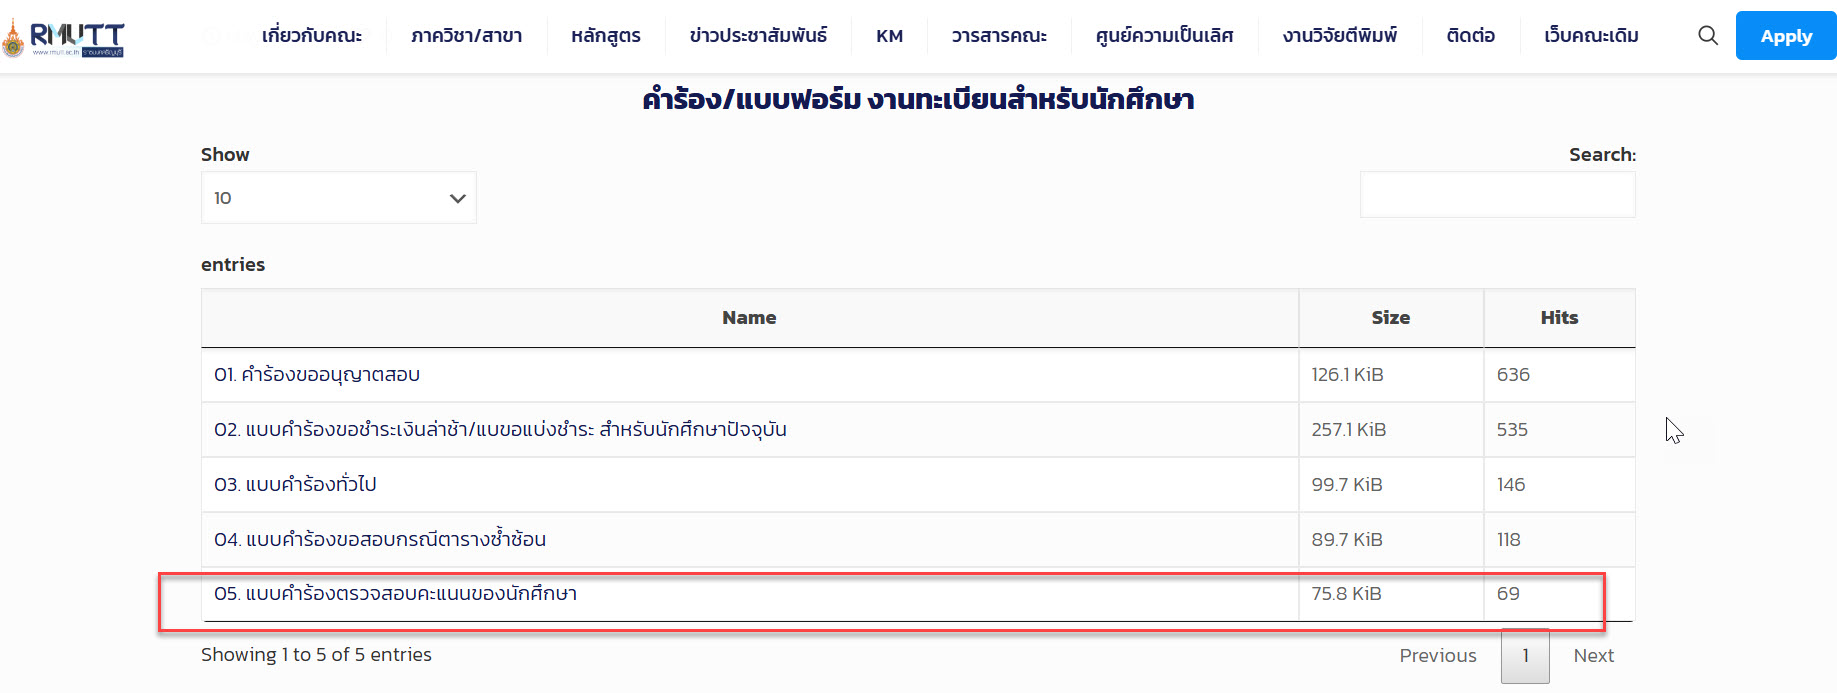
\includegraphics[width=\textwidth]{Pic4.2-2.jpg}
		\caption{เว็บไซต์สำหรับดาวน์โหลดเอกสารข้อร้องเรียนหรืออุทธรณ์ผลการประเมิน}
\end{figure}
\\
\noindent
\newpage
ขั้นตอนการอุทธรณ์ผลการประเมิน
\begin{enumerate}
\item ยื่นคำร้องที่เจ้าหน้าที่ธุรการสาขาในวันและเวลาราชการ โดยวันสุดท้ายที่จะสามารถยื่นเรื่องได้จะต้องไม่เกิน 7 วันทำการนับจากวันสุดท้ายที่คณะส่งค่าระดับคะแนนตามกำหนดการของสำนักส่งเสริมวิชาการและงานทะเบียน (สวท.)
\item ขอดูได้เป็นรายบุคคลเท่านั้น โดยธุรการสาขานัดหมายนักศึกษาให้มาดูเอกสารประกอบการตรวจสอบหลังจากยื่นคำร้องในวันทำการถัดไปในกรณีที่ยื่นคำร้องก่อนเวลา 12.00 น. หรือในอีก 2 วันทำการถัดไปในกรณีที่ยื่นคำร้องหลังเวลา 12.00 น.
\item ธุรการสาขาประสานงานกับคณะกรรมการการอุทธรณ์ที่ได้รับการแต่งตั้งจากสาขาวิชา ซึ่งคณะกรรมการชุดดังกล่าวไม่มีส่วนเกี่ยวข้องกับอาจารย์ผู้สอนรายวิชาที่นักศึกษาได้ยื่นเรื่องอุทธรณ์ เพื่อจัดเตรียมเอกสารและนัดหมายเวลาสำหรับการเข้าตรวจสอบคะแนนของนักศึกษา ทั้งนี้ให้ธุรการสาขาดำเนินการหลังจากได้รับคำร้องจากนักศึกษาทันที
\item ผู้สอนจัดเตรียมกระดาษคำตอบของนักศึกษาที่ยื่นคำร้อง เฉลย และเกณฑ์การให้คะแนนของข้อสอบในรายวิชา
นั้น ๆ ให้แก่คณะกรรมการการอุทธรณ์ที่ได้รับการแต่งตั้งจากสาขาวิชา
\item นักศึกษาเข้าพบธุรการสาขา และคณะกรรมการการอุทธรณ์ที่ได้รับการแต่งตั้งจากสาขาวิชาเพื่อตรวจสอบเอกสาร โดยไม่อนุญาตให้จด บันทึกภาพถ่ายหรือวีดีโอขณะทำการตรวจสอบเอกสาร
\item หากนักศึกษาไม่ยอมรับผลคะแนนสอบหลังจากทำการตรวจสอบคะแนนแล้ว ให้ธุรการสาขาส่งเรื่องต่อ
ให้กับงานทะเบียนและวัดผล ฝ่ายวิชาการ เพื่อดำเนินการแต่งตั้งคณะกรรมการเพื่อตรวจสอบการให้คะแนนของ
ผู้สอนอีกครั้ง โดยมีคณะกรรมการในการดำเนินการ 3 ท่าน คือ
\begin{enumerate}[label=\arabic*),leftmargin=1cm]
\item รองคณบดีฝ่ายวิชาการ 
\item หัวหน้างานทะเบียนและวัดผล
\item หัวหน้าภาควิชา/สาขาวิชา หรือตัวแทนคณะกรรมการหลักสูตรที่เกี่ยวข้อง
\end{enumerate}
\item งานทะเบียนและวัดผล ฝ่ายวิชาการ ดำเนินการนัดหมายคณะกรรมการในการตรวจสอบ อาจารย์ผู้สอนนักศึกษา และธุรการสาขา เพื่อดำเนินการตรวจสอบต่อไป และดำเนินการให้เสร็จสิ้นภายใน 3 วันทำการ
\end{enumerate}
ผลการดำเนินการในปีการศึกษา 2567 พบว่าไม่มีนักศึกษาดำเนินการอุทธรณ์ผลการประเมิน 

\begin{doclist}
	\docitem{แบบคำร้องขอตรวจสอบคะแนนของนักศึกษา}
\end{doclist}


%%%%%%% 4.3 %%%%%%%%%%%%%%%%%%%%%%%
\subcriteria{The assessment standards and procedures for student progression and degree completion, are shown to be explicit, communicated to students, and applied consistently.}
หลักสูตรได้กำหนดกระบวนการในการติดตามการประเมินผลและการสำเร็จการศึกษาของนักศึกษาไว้อย่างเป็นระบบและชัดเจน โดยยึดตามข้อบังคับของมหาวิทยาลัยเทคโนโลยีราชมงคลธัญบุรี ว่าด้วยการศึกษาระดับปริญญาตรี พ.ศ. 2556 และเป็นไปตามกรอบมาตรฐานคุณวุฒิระดับอุดมศึกษาแห่งชาติ (TQF) เพื่อให้มั่นใจว่าบัณฑิตทุกคนมีคุณภาพและเป็นไปตามผลลัพธ์การเรียนรู้ระดับหลักสูตร (PLOs) ของหลักสูตร ดังรายละเอียดต่อไปนี้ 
\begin{enumerate}
	\item หลักสูตรแต่งตั้งอาจารย์ที่ปรึกษาสำหรับดูแลนักศึกษาแต่ละชั้นปี ในการกำกับติดตามเกี่ยวกับ
	\begin{enumerate}[label=\arabic*),leftmargin=0.7cm]
		\item ด้านการลงทะเบียนเรียน
		\begin{itemize}
			\item ในภาคการศึกษาปกตินักศึกษาต้องลงทะเบียนเรียนไม่ต่ำกว่า 9 หน่วยกิต และไม่เกิน 22 หน่วยกิต สำหรับภาคฤดูร้อน นักศึกษาจะลงทะเบียนได้ไม่เกิน 9 หน่วยกิต หากไม่เป็นไปตามเกณฑ์นี้ให้ขออนุมัติต่อคณบดี และทำได้เพียง 1 ภาคการศึกษาเท่านั้นในการศึกษาตลอดหลักสูตร
			\item รายวิชาที่ลงทะเบียนในแต่ละภาคเรียนต้องเป็นไปตามแผนการศึกษา ในกรณีที่นักศึกษามีผลการเรียนไม่ถึง 2.00 นักศึกษาจะต้องได้รับการปลดล็อคและรับคำปรึกษาจากอาจารย์ที่ปรึกษาในการลงทะเบียนเรียน
			\item สำหรับนักศึกษาที่ต้องลงทะเบียนเรียนไม่เป็นไปตามแผนการเศึกษาที่กำหนด อาจารย์ที่ปรึกษาจะให้คำแนะนำปรึกษาการวางแผนลงทะเบียนเรียนและกำกับติดตามให้นักศึกษาลงทะเบียนเรียนรายวิชาให้ครบตามแผนการศึกษาของหลักสูตร
		\end{itemize}
		\item ด้านผลการศึกษา\\
		อาจารย์ที่ปรึกษากำกับติดตามผลการเรียนของนักศึกษาผ่านระบบงานทะเบียนทางเว็บไซต์ (www.oreg.rmutt.ac.th) เพื่อ
		\begin{itemize}
			\item ดูแนวโน้มผลการเรียนและแนะนำในการวางแผนการศึกษา
			\item เฝ้าระวังการพ้นสภาพตามเกณฑ์ ซึ่งมีเกณฑ์การพ้นสภาพดังนี้\\
			
			\begin{tabular}{|c|c|}
				\hline
				\textbf{หน่วยกิตสะสม}& \textbf{พ้นสภาพเมื่อได้ระดับคะแนน}\\\hline
				น้อยกว่า 30 หน่วยกิต& น้อยกว่า 1.00\\\hline
				30-59 หน่วยกิต& น้อยกว่า 1.50\\\hline
				60 หน่วยกิตขึ้นไป &  น้อยกว่า 1.75\\\hline
				ครบหลักสูตร &  น้อยกว่า 1.90\\\hline
			\end{tabular}\\
			หมายเหตุ รายวิชาที่ลงทะเบียนเรียนซ้ำ ให้นับหน่วยกิตเฉพาะที่ได้ระดับคะแนนดีที่สุดเพียงครั้งเดียว และการนับหน่วยกิตสะสมสำหรับเกณฑ์การพ้นสภาพเนื่องจากผลการศึกษาให้นับหน่วยกิตทุกรายวิชาที่ได้ค่าระดับคะแนน ยกเว้น W I S และ U
		\end{itemize}
		\item ด้านการสำเร็จการศึกษาตามหลักสูตร
		\begin{itemize}
			\item ต้องศึกษารายวิชาให้ครบตามโครงสร้างหลักสูตร
			\item มีจำนวนหน่วยกิตสะสมไม่ต่ำกว่า 137 หน่วยกิต และได้ค่าระดับคะแนนเฉลี่ยสะสมไม่ต่ำกว่า 2.00 จากระบบ 4 ระดับคะแนนหรือเทียบเท่า
			\item ใช้ระยะเวลาไม่เกิน 2 เท่าของระยะเวลาการศึกษาที่กำหนดไว้ในหลักสูตร ทั้งนี้ไม่นับระยะเวลาการลาพักการศึกษาด้วย
			\item มีผลการทดสอบภาษาอังกฤษเป็นไปตามเกณฑ์ที่มหาวิทยาลัยกำหนด
			\item มีคุณสมบัติอื่น ๆ ตามข้อบังคับของมหาวิทยาลัยเทคโนโลยีราชมงคลธัญบุรี ว่าด้วยการศึกษาระดับปริญญาตรี พ.ศ. 2550 และฉบับเพิ่มเติม พ.ศ. 2556
		\end{itemize}
	\end{enumerate}	
	\item หลักสูตรมีการสื่อสารให้นักศึกษาทราบถึงเกณฑ์การประเมินผลและการสำเร็จการศึกษาอย่างสม่ำเสมอผ่านช่องทาง ดังนี้
	\begin{itemize}
		\item การปฐมนิเทศนักศึกษาใหม่\\อาจารย์ที่ปรึกษาและคณาจารย์ในหลักสูตรฯ จะชี้แจงภาพรวมของหลักสูตร เกณฑ์การวัดผลและประเมินผล และเงื่อนไขการสำเร็จการศึกษาให้นักศึกษาใหม่ทราบทุกปีการศึกษา
		\item ระบบงานทะเบียน\\ นักศึกษาสามารถเข้าถึงรายละเอียดหลักสูตร ข้อบังคับต่างๆ และตรวจสอบผลการเรียนของตนเองได้ตลอดเวลาผ่านทางเว็บไซต์ของระบบงานทะเบียน (www.oreg.rmutt.ac.th)
		\item อาจารย์ที่ปรึกษา\\ให้คำแนะนำ ดูแล และให้คำปรึกษาแก่นักศึกษาในเรื่องการวางแผนการเรียนและติดตามผลการเรียนอย่างสม่ำเสมอ
	\end{itemize}
\end{enumerate}

\begin{doclist}
	\docitem{หลักสูตรวิทยาศาสตรบัณฑิต สาขาวิชาคณิตศาสตร์ประยุกต์ (หลัก\newline สูตรปรับปรุง พ.ศ. 2564)}
	\docitem{ข้อบังคับ ระเบียบ และประกาศ ที่เกี่ยวข้องกับการจัดการศึกษาของมหาวิทยาลัยเทคโนโลยีราชมงคลธัญบุรี}
	\docitem{คู่มือนักศึกษา}
\end{doclist}

%%%%%%% 4.4 %%%%%%%%%%%%%%%%%%%%%%%
\subcriteria{The assessments methods are shown to include rubrics, marking schemes, timelines, and regulations, and these are shown to ensure validity, reliability, and fairness in assessment.}
%%%%%%%%%%%%%%%%%%%%%%%%%%%%%%%%%%
เพื่อให้เกิดความมั่นใจว่าการวัดและประเมินผลนักศึกษามีความถูกต้อง เชื่อถือได้ และเป็นธรรม หลักสูตรมี​การดำเนินการดังนี้
\begin{enumerate}
\item ทุกรายวิชามีการแจ้งรายละเอียดของรายวิชา (มคอ.3) ซึ่งมีรายละเอียดของกำหนดการและเกณฑ์ในการวัดและประเมินผลของรายวิชาให้นักศึกษาทราบและแจกประมวลรายวิชา (Course Syllabus) ของรายวิชาที่มี Qr-code ของ มคอ.3 ให้กับนักศึกษาในคาบแรกของการเรียนการสอน
\item นักศึกษาทุกคนที่ลงทะเบียนเรียนในรายวิชา จะได้รับการประเมินผลการเรียนในรูปแบบ วิธีการ และเกณฑ์เดียวกัน
\item ข้อสอบสำหรับการประเมินผลในแต่ละรายวิชา อาจารย์ผู้สอนในรายวิชาเป็นผู้ออกข้อสอบ ในกรณีที่มีผู้สอนร่วมกัน อาจารย์ผู้สอนจะออกข้อสอบร่วมกันพร้อมทั้งตรวจสอบความถูกต้องของข้อสอบ สำหรับการตรวจข้อสอบแบบอัตนัย อาจารย์ผู้สอนจะทำแนวเฉลยข้อสอบหรือ marking schemes เพื่อให้อาจารย์ผู้สอนทุกท่านนำไปเป็นแนวทางในการตรวจข้อสอบ ดังตัวอย่าง marking schemes ของข้อสอบรายวิชาแคลคูลัส 1 (
รูปภาพที่ \ref{Picture:Marking Schemes})
\begin{figure}[h!]
	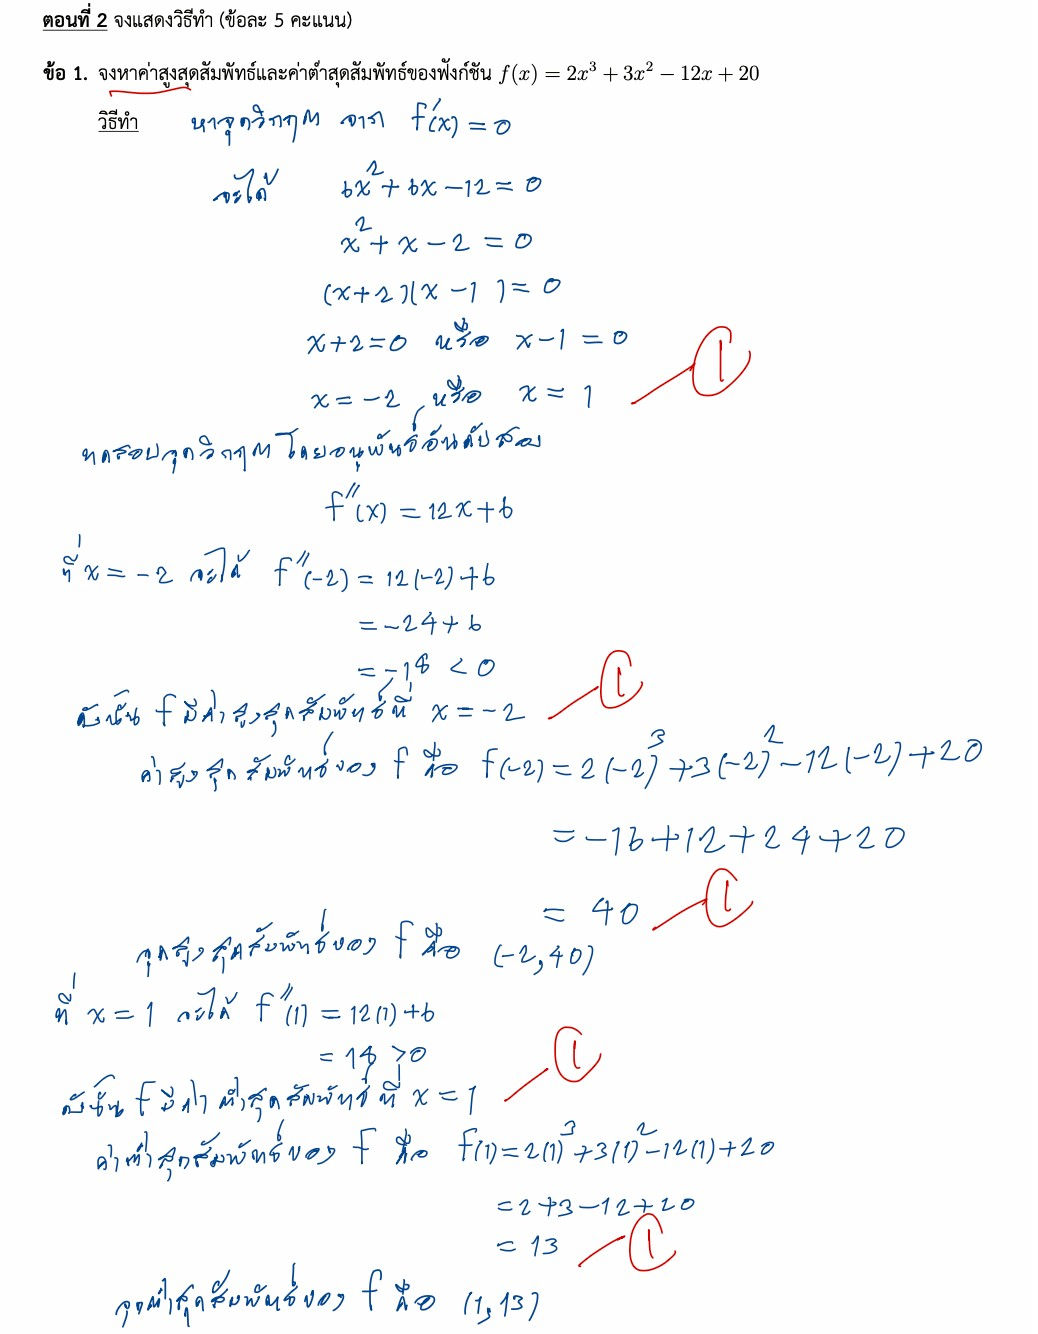
\includegraphics[width=\textwidth]{Calculus Points}\\
	\caption{ตัวอย่าง Marking Schemes ของข้อสอบรายวิชา Calculus 1}
	\label{Picture:Marking Schemes}
\end{figure}
\item สำหรับรายวิชาชีพที่มีการประเมินผลการนำเสนอผลงาน ผู้สอนมีการจัดทำ Scoring Rubrics สำหรับให้คะแนนทุกรายวิชาดังตาราง \ref{table: Scoring Rubrics}

\renewcommand{\arraystretch}{1.5} % เพิ่มความสูงบรรทัดให้อ่านง่ายขึ้น

\begin{longtable}{|p{3cm}|p{1.8cm}|p{1.8cm}|p{1.8cm}|p{1.8cm}|p{1.8cm}|p{1cm}|}
		\caption{เกณฑ์การให้คะแนน (Scoring Rubrics) สำหรับการประเมินผลการนำเสนอ}
	\label{table: Scoring Rubrics}\\
	\hline
	\centering\textbf{รายการประเมิน}&\multicolumn{5}{c|}{\textbf{ระดับคะแนน}}&\textbf{คะแนน\newline ที่ได้}\\ \cline{2-6}
	& \centering\textbf{5} & \centering\textbf{4} & \centering\textbf{3} & \centering\textbf{2} & \centering\textbf{1} &  \\
	\hline
	\endfirsthead
	
	\caption{(ต่อ) เกณฑ์การให้คะแนน (Scoring Rubrics) สำหรับการประเมินผลการนำเสนอ }\\
	\hline
\centering\textbf{รายการประเมิน}&\multicolumn{5}{c|}{\textbf{ระดับคะแนน}}&\textbf{คะแนน\newline ที่ได้}\\ \cline{2-6}
& \centering\textbf{5} & \centering\textbf{4} & \centering\textbf{3} & \centering\textbf{2} & \centering\textbf{1} &  \\
\hline
	\endhead
					\vspace{-0.55cm}
	\begin{itemize}
		\item[1.]ความถูกต้อง \newline ของเนื้อหา \newline (30\%) 
	\end{itemize}
 & 
	ข้อมูลถูกต้อง\newline ครบถ้วน \newline น่าเชื่อถือสูง \newline อ้างอิง\newline ได้ชัดเจน &
	ข้อมูลถูกต้อง น่าเชื่อถือ อ้างอิงได้  &
	ข้อมูลถูกต้องเป็นส่วนใหญ่ มีข้อผิดพลาดเล็กน้อย &
	ข้อมูลมี\newline ข้อผิดพลาดหลายจุด \newline ไม่น่าเชื่อถือบางส่วน&
	ข้อมูลมี\newline ข้อผิดพลาดอย่างมาก \newline ไม่น่าเชื่อถือ&
	\\
	\hline
				\vspace{-0.55cm}
	\begin{itemize}
		\item[2.]การนำเสนอ \newline(20\%)
	\end{itemize}
	& 
	การนำเสนอมีความน่าสนใจอย่างยิ่ง\newline สามารถดึงดูดความสนใจของ\newline ผู้ชมได้อย่างยอดเยี่ยม &
	การนำเสนอมีความน่าสนใจ\newline ดึงดูดความสนใจของ\newline ผู้ชมได้ดี &
	การนำเสนอค่อนข้าง\newline น่าเบื่อ\newline ไม่สามารถดึงดูดความสนใจได้ตลอด&
	การนำเสนอไม่น่าสนใจ ไม่ดึงดูดผู้ชม &
	การนำเสนอไม่น่าสนใจและไม่ดึงดูดผู้ชมเลย &
	\\
	\hline
			\vspace{-0.55cm}
	\begin{itemize}
		\item[3.]การใช้สื่อ\newline ประกอบ\newline(15 \%)
	\end{itemize}
  &
	อธิบายและเชื่อมโยงสื่อประกอบ\newline กับการ\newline นำเสนอได้อย่างกลมกลืน ช่วยให้ผู้ชมเข้าใจเนื้อหาได้ดียิ่งขึ้น &
	อธิบายและเชื่อมโยงสื่อประกอบกับการนำเสนอได้ดี &
	อธิบายสื่อประกอบบ้าง แต่ยังไม่เชื่อมโยงกับการ\newline นำเสนอ &
	ไม่มีการอธิบาย \newline หรืออธิบายสื่อประกอบได้ไม่ดี &
	ไม่มีการอธิบาย \newline หรืออธิบายสื่อประกอบได้ไม่ดีเลย &
	 \\
	\hline
		\vspace{-0.55cm}
	\begin{itemize}
		\item[4.]การตอบคำถาม\newline ข้อซักถาม\newline (30\%)
	\end{itemize}
 &
	ตอบคำถามได้อย่างยอดเยี่ยม มั่นใจ\newline มีเหตุผลประกอบที่ดี และสามารถจัดการกับ\newline คำถามยากๆ ได้ &
ตอบคำถามได้ดี มั่นใจ \newline และมีเหตุผลประกอบ &
	ตอบคำถามได้บ้าง แต่ยัง\newline ไม่มั่นใจ หรือใช้เวลานาน &
	ไม่สามารถตอบคำถามได้ หรือตอบ\newline ผิด &
	ไม่สามารถตอบคำถามได้เลย \newline หรือตอบผิดทั้งหมด &
\\
	\hline
	\vspace{-0.55cm}
	\begin{itemize}
		\item[5.]การบริหารเวลา\newline(5\%)
	\end{itemize}
	&
	บริหารเวลาได้อย่างยอดเยี่ยมนำเสนอได้ครบถ้วนตามเวลาที่กำหนด และมีเวลาสำหรับตอบคำถาม  \newline ได้อย่างเหมาะสม &
	บริหารเวลาได้ดี นำเสนอได้ตามเวลาที่กำหนด &
	ใช้เวลาพอดี แต่บางส่วนรีบเร่ง หรือใช้เวลากับบางประเด็นมากเกินไป &
	ใช้เวลา \newline ไม่เหมาะสม น้อยเกินไป หรือเกินเวลามาก &
ใช้เวลา \newline ไม่เหมาะสม  \newline อย่างมาก น้อยเกินไป หรือเกินเวลามากเกินไป &
	\\
	\hline
	
\end{longtable}


\item การแจ้งผลการเรียนของรายวิชาหลังเสร็จสิ้นภาคการศึกษา อาจารย์ผู้สอนเป็นผู้รวบรวมคะแนนของนักศึกษาและจัดทำเกรดตามเกณฑ์ที่กำหนดไว้ใน มคอ.3 และนำเสนอต่อที่ประชุมสาขาวิชาคณิตศาสตร์เพื่อพิจารณา หลังจากนั้นนำเข้าสู่การพิจารณาโดยคณะกรรมการบริหารคณะและคณะกรรมการประจำคณะ หากผ่านการพิจารณาของคณะกรรมการบริหารคณะและคณะกรรมการประจำคณะ ไม่มีปัญหาใด อาจารย์ผู้รับผิดชอบในการ submit เกรดของสาขาวิชา จะดำเนินการ submit เกรดของนักศึกษาทุกรายวิชา ผ่านระบบ OREG ของมหาวิทยาลัย

\end{enumerate}
%%%%%%%%%%%%%%%%%%%%%%%%%%%%%%%%%%%%
\begin{doclist}
	\docitem{Marking Schemes ของข้อสอบรายวิชา Calculus 1 }
	\docitem{Scoring Rubrics สำหรับการประเมินผลการนำเสนอ}
\end{doclist}



%%%%%%% 4.5 %%%%%%%%%%%%%%%%%%%%%%%
\subcriteria{The assessment methods are shown to measure the achievement of the expected learning outcomes of the programme and its courses.}
%%%%%%%%%%%%%%%%%%%%%%%%%%%%%%%5
หลักสูตรมีวิธีการวัดและประเมินการบรรลุความสำเร็จตามผลลัพธ์การเรียนรู้ระดับรายวิชา (CLOs) และผลลัพธ์การเรียนรู้ระดับหลักสูตร (PLOs) ดังนี้
\begin{enumerate}
	\item วิธีการวัดและประเมินผลการบรรลุผลลัพธ์การเรียนรู้ระดับรายวิชา (CLOs)
	\begin{itemize}
		\item[1)] การประเมินผลโดยผู้สอน ผ่านการวัดผลของรายวิชา
		\item[2)] การประเมินตนเองของนักศึกษา โดยให้นักศึกษาทำแบบประเมินการบรรลุ CLOs เมื่อสิ้นภาคการศึกษา
	\end{itemize}
	\item วิธีการวัดและประเมินผลการบรรลุผลลัพธ์การเรียนรู้ระดับหลักสูตร (PLOs)
	\begin{itemize}
		\item[1)] การประเมินผลโดยตรงผ่านผลงานและการวัดผลในชั้นเรียนโดยผู้สอนของทุกรายวิชาที่รับผิดชอบการบรรลุแต่ละ PLOs 
		\item[2)] การประเมินตนเองของนักศึกษาชั้นปีที่ 4 ผ่านแบบประเมินการบรรลุ PLOs เมื่อสิ้นภาคการศึกษา 2/\printyear{} 
		\item[3)] การประเมินความพึงพอใจของผู้ใช้บัณฑิตซึ่งเป็นมุมมองสะท้อนกลับจากผู้มีส่วนได้ส่วนเสียภายนอก
	\end{itemize}
	ซึ่งมีรายละเอียดและผลการประเมินดัง criterion 1.5
\end{enumerate}
\begin{doclist}
	\docitem{ผลการประเมินการบรรลุผลลัพธ์การเรียนรู้ระดับหลักสูตร (PLOs)}
	\docitem{ผลการประเมินการบรรลุผลลัพธ์การเรียนรู้ระดับรายวิชา (CLOs)}
\end{doclist}

%%%%%%% 4.6 %%%%%%%%%%%%%%%%%%%%%%%
\subcriteria{Feedback of student assessment is shown to be provided in a timely manner.}

หลักสูตรมีนโยบายให้ผู้สอนในทุกรายวิชาดำเนินการให้ข้อมูลย้อนกลับ (Feedback) แก่นักศึกษาอย่างสม่ำเสมอ ภายหลังการประเมินผล เพื่อให้นักศึกษาได้รับข้อมูลที่ชัดเจนเกี่ยวกับผลการเรียน จุดแข็ง จุดที่ควรปรับปรุง และแนวทางการพัฒนาในครั้งต่อไป โดยมีรูปแบบการดำเนินการที่สำคัญ ดังนี้
\begin{enumerate}
	\item  อาจารย์ผู้สอนทุกรายวิชามีการแจ้งผลการประเมิน และให้ข้อมูลย้อนกลับ (Feedback) แก่นักศึกษา
	\begin{itemize}
		\item คะแนนสอบกลางภาค/คะแนนทดสอบย่อย\\
		มีการเฉลยแบบทดสอบ ให้ข้อเสนอแนะ ข้อควรปรับปรุง เพื่อปรับปรุงพัฒนาตนเอง เตรียมพร้อมสำหรับการสอบในครั้งถัดไป หรือวางแผนถอนรายวิชา
		\item คะแนนชิ้นงาน \\มีการให้ข้อเสนอแนะข้อควรปรับปรุง เพื่อพัฒนาชิ้นงาน
		\item คะแนนการนำเสนอ \\มีการให้ข้อเสนอแนะข้อควรปรับปรุงในการนำเสนอ
	\end{itemize} 
	\item การให้ข้อมูลย้อนกลับในรายวิชาโครงงานด้านคณิตศาสตร์ประยุกต์\\
นักศึกษาจะได้รับข้อมูลย้อนกลับจากอาจารย์อย่างต่อเนื่อง ทั้งในระหว่างการดำเนินโครงงานและหลังการนำเสนอ โดยเฉพาะข้อเสนอแนะเพื่อพัฒนาแนวคิด วิธีการและผลลัพธ์ของโครงงาน
	\item การให้ข้อมูลย้อนกลับในรายวิชาสัมมนาทางคณิตศาสตร์ประยุกต์\\
ในรายวิชาสัมมนาทางคณิตศาสตร์ หลักสูตรได้จัดให้มีคณะกรรมการประเมินการนำเสนอการถอดบทเรียนและอาจารย์ที่ปรึกษา เพื่อให้คำแนะนำเชิงวิชาการและข้อเสนอแนะเฉพาะบุคคลระหว่างการนำเสนอของนักศึกษา โดยกรรมการจะมีการสอบถาม วิเคราะห์ และเสนอแนวทางพัฒนาอย่างเป็นระบบ เพื่อใหนักศึกษาสามารถนำ feedback ที่ได้รับไปปรับปรุงในการนำเสนอครั้งถัดไป
	\end{enumerate}


%%%%%%% 4.7 %%%%%%%%%%%%%%%%%%%%%%%
\subcriteria{The student assessment and its processes are shown to be continuously reviewed and improved to ensure their relevance to the needs of industry and alignment to the expected learning outcomes.}

หลักสูตรมีการทบทวนกลไกการวัดและประเมินผลการเรียนรู้ของนักศึกษาอย่างต่อเนื่องโดยมุ่งเน้นให้การวัดและประเมินผลมีความสอดคล้องกับผลลัพธ์การเรียนรู้ระดับรายวิชา (CLOs) วัตถุประสงค์ของรายวิชา และความต้องการของภาคอุตสาหกรรมในปัจจุบัน โดย 
\begin{enumerate}
	\item เก็บรวบรวมข้อมูลข้อเสนอแนะจากอาจารย์ผู้สอน \\ โดยอาจารย์ผู้สอนให้ข้อเสนอแนะในการปรับปรุงการประเมินผลไว้ใน มคอ.5 หลังจากนั้นอาจารย์ผู้รับผิดชอบรายวิชาและอาจารย์ผู้สอนประชุมร่วมกัน
	เพื่อพิจารณาข้อเสนอแนะและนำมาใช้ในการปรับปรุงการวัดและประเมินผลในภาคเรียนถัดไป
	\item เก็บรวบรวมข้อเสนอแนะจากนักศึกษา\\ โดยอาจารย์ผู้สอนรวบรวมข้อมูลเสนอแนะจากนักศึกษาเมื่อสิ้นภาคการศึกษา ในกรณีที่นักศึกษามีข้อเสนอแนะเพิ่มเติมเกี่ยวกับการวัดและประเมินผล หลักจากนั้นอาจารย์ผู้สอนนำข้อเสนอแนะที่เป็นประโยชน์เสนอต่อที่ประชุมอาจารย์ผู้สอนและผู้รับผิดชอบรายวิชา เพื่อเป็นข้อมูลในการปรับปรุงการประเมินผลรายวิชาในภาคการศึกษาถัดไป
	\item การทวนสอบฯ\\
	หลักสูตรมีการทวนสอบผลสัมฤทธิ์ของนักศึกษาตามผลลัพธ์การเรียนรู้ระดับรายวิชา (CLOs) ของทุกรายวิชาชีพที่เปิดสอนในแต่ละภาคเรียน โดย
	\begin{itemize}
		\item แต่งตั้งคณะกรรมการทวนสอบฯ
		\item คณะกรรมการทวนสอบฯ ดำเนินการทวนสอบหลังสิ้นภาคเรียน
		\item คณะกรรมการทวนสอบฯ รายงานผลการทวนสอบให้หลักสูตรทราบ และแจ้งผลการทวนสอบพร้อมทั้งข้อเสนอแนะให้กับอาจารย์ผู้รับผิดชอบรายวิชา และอาจารย์ผู้สอนทราบเพื่อนำไปปรับปรุงการวัดและประเมินผลในภาคการศึกษาถัดไป
	\end{itemize}
	\item เก็บข้อมูลข้อเสนอแนะจากภาคอุตสาหกรรม\\
	ในแต่ละปีการศึกษา หลักสูตรมีการเก็บรวบรวมข้อมูลข้อเสนอแนะจากภาคอุตสาหกรรมจากหลายช่องทาง เช่น การสัมภาษณ์สถานประกอบการที่นักศึกษาออกฝึกประสบการวิชาชีพ ข้อเสนอแนะจากผู้ทรงคุณวุฒิจากหน่วยงานภายนอกที่มาร่วมพิจารณาเกรดในการประชุมคณะกรรมการประจำคณะ
\end{enumerate}

ในปีการศึกษา 2567  มีรายวิชาที่เปิดสอนในหลักสูตรจำนวน 31 รายวิชา แบ่งเป็น
\begin{enumerate}
	\item[] - ภาคเรียนที่ 1/2567 จำนวน 11 รายวิชา
	\item[] - ภาคเรียนที่ 2/2567 จำนวน 20 รายวิชา
\end{enumerate}
พบว่าทุกรายวิชามีการออกแบบการวัดและการประเมินผลที่สอดคล้องกับผลลัพธ์การเรียนรู้ระดับรายวิชา (CLOs) นอกจากนี้ จากการสัมภาษณ์สถานประกอบการที่นักศึกษาออกฝึกประสบการณ์วิชาชีพ ในภาคเรียนที่ 1 ปีการศึกษา 2567 ทางสถานประกอบการมีข้อเสนอแนะว่าหลักสูตรควรเพิ่มการประเมินผลในลักษณะที่นักศึกษาได้เลือกสถานการณ์ของปัญหา เลือกวิธีวิเคราะห์และแก้ปัญหาด้วยตนเอง พร้อมทั้งนำเสนอแนวคิดและวิธีการแก้ปัญหานั้นๆ เพื่อส่งเสริมให้นักศึกษาได้ฝึกคิดวิเคราะห์และนำเสนอ และเตรียมพร้อมสำหรับการปฏิบัติงานจริงในสถานประกอบการ ที่ต้องมีการคิดการวิเคราะห์และการนำเสนองานในส่วนที่ตนเองรับผิดชอบอยู่เสมอ ซึ่งถือเป็นทักษะที่สำคัญมากในการทำงานที่ทางสถานศึกษาควรส่งเสริม

หลักสูตรได้นำข้อเสนอแนะมาปรับปรุงการดำเนินงานในภาคเรียนที่ 2/2567 ในรายวิชาการตัดสินใจอย่างชาญฉลาดด้วยกำหนดการเชิงคณิตศาสตร์ โดยเพิ่มกิจกรรมการประเมินผลตามข้อเสนอแนะจากสถานประกอบการ โดยเปิดโอกาสให้นักศึกษาเลือกปัญหาที่เป็นไปได้จากสถานการณ์จริง และออกแบบวิธีการแก้ปัญหาด้วยตนเองพร้อมนำเสนอ




\begin{doclist}
	\docitem{รายงานผลการทวนสอบปีการศึกษา 2567}
	\docitem{หลักฐานการปรับปรุงการประเมินผลรายวิชาการตัดสินใจอย่างชาญฉลาดด้วยกำหนดการเชิงคณิตศาสตร์}
\end{doclist}


